\chapter{Background Research \& Notation}
\label{chapter2}
\section{Markov Decision Processes}
The Markov Property states that the future is conditionally independent of the past given the present. A sequential decision-making problem that satisfies the Markov Property is known as a Markov Decision Problem, and can be modelled by a Markov Decision Process (MDP) \citep{10.5555/528623}. Where an agent is able to fully observe its state, the problem can be modelled as an MDP. Conversely, where an agent can only partially observe its state, the problem can be modelled by a Partially Observable Markov Decision Process (POMDP).
Consider an agent playing a perfect information game, such as Chess or Go, the agent (and its opponent) are able to fully observe the state of the game with ease. However, a robot navigating through a maze may not be able to observe its exact state due to uncertainty in its sensors.
Furthermore, an MDP can be stationary or non-stationary which refer to whether its dynamics stay the same, or change temporally.
An MDP that contains absorbing states, that is any state that upon entering the task terminates, then it is said to be episodic.
\\Within this work we assume that the agent is fully able to observe its state, the environment is stationary and can be discretised in some way and tasks are episodic.
% and tasks are episodic (there exist some terminal states which indicate the end of a task); 
Hence we consider \textbf{stationary}, \textbf{finite}, \textbf{undiscounted} MDPs.
Thus, an MDP is a 5-tuple: $\text{MDP} = (S,A,T,R)$ where:
\begin{itemize}
    \item $S$ is a finite set of states.
    \item $A$ is a finite set of actions.
    \item $T : S \times A \times S \rightarrow [0,1]$ is the transition function, which determines the probability of transitioning from a state $s \in S$ to $s' \in S$ with an action $a \in A$.
    \item $R:S \times A \times S \rightarrow \mathbb{R}$ is the reward function, which determines the reward signal, $r \in \mathbb{R}$ received by the agent from transitioning from a state $s \in S$ to $s' \in S$ with the action $a \in A$. This reward is extrinsic to the agent; it comes from the environment.
\end{itemize}
The transition function, $T$ is a key indicator about the nature of the environment.
If $\forall s,s' \in S, \forall a \in A$, $T(s,a,'s) \in \{0,1\}$, then the environment is deterministic, otherwise it is stochastic.
A deterministic environment is one which there is no variance in the outcomes of action in a given state; taking the same action in the same state always produces the same outcome. Whereas a stochastic (or non-deterministic) environment has uncertainty associated with transitions.
\subsection{Policies, Value and Quality}
% The goal of a decision-making agent acting in an MDP is to maximise the cumulative reward it receives over time - to maximise the return:
A policy, denoted by $\pi$, is a mapping of states to actions that describes a behaviour within an MDP. The desired behaviour within an MDP is to maximise the cumulative reward, this is known as the optimal policy and denoted $\pi^*$. The cumulative reward is given by:
\begin{equation}
\label{eqn:return}
G_t = \sum_{k=t+1}^TR_{k}
\end{equation}
which represents the cumulative reward received from time $t$ to some finite time $T$.
A Value Function, or state-value function, denoted $V^\pi(s)$, measures the expected cumulative reward that can be received starting in each state $s \in S$ and following a policy $\pi$:
\begin{equation}
\label{eqn:vs}
    V^\pi(s) = \mathbb{E}^\pi\Bigg[G_t | s_t = s\Bigg] = \mathbb{E}^\pi\ \Bigg[\sum_{k=t+1}^TR_{k} | s_t = s \Bigg]
\end{equation}
Where $\mathbb{E}$ represents the expected value that the agent follows $\pi$, $t$ is an arbitrary time step and $T$ is a finite time horizon.
The optimal Value Function, $V^*$, is the one that is maximum for every $s \in S$ and is given by:
\begin{equation}
\label{eqn:vsm}
    V^*(s) = \max_\pi V_\pi(s) = \max_a\sum_{s'}T(s,a,s')[R(s,a,s')+V^*(s')]
\end{equation}
Similarly, a Q-Function, or action-value function, denoted $Q^\pi(s,a)$, measures the expected cumulative reward that can be received starting in each state $s \in S$, taking an action $a \in A$ and thereafter following a policy $\pi$:
\begin{equation}
\label{eqn:qsa}
Q^\pi(s,a) = \mathbb{E}^\pi\Bigg[G_t | s_t = s,a_t = a\Bigg] = \mathbb{E}^\pi\Bigg[\sum_{k=t+1}^TR_{k}|s_t=a, a_t = a\Bigg]
\end{equation}
Where $\mathbb{E}$ represents the expected value that the agent follows $\pi$, $t$ is an arbitrary time step and $T$ is a finite time horizon.
The optimal Q-Function, $Q^*$, is the one that is maximum for every $s,a \in S \times A$ and is given by:
\begin{equation}
\label{eqn:qsn}
Q^*(s,a) = \sum_{s'}T(s,a,s')[R(s,a,s')+\max_{a'}Q^*(s',a')]
\end{equation}
An interesting observation is that $\pi^*$ can be derived from both $V^*$ and $Q^*$. In the case of $V^*$, $\pi^*$ can be derived by determining at each state, which actions yield the next state with the maximum value. In the case of $Q^*$, $\pi^*$ can be derived by simply taking the action with the highest Q-value at each state \cite{Sutton1998}.

% The optimal value function, $V^*(s)$, is the one that is maximum for every $s \in S$, it also happens to correspond to $\pi^*$.
% Similarly, a Q-Function, denoted $Q^\pi(s,a)$, measures the expected cumulative reward that can be received starting in each state $s \in S$ and taking an action $a \in A$ and thereafter following $\pi$. The optimal quality function, $Q^*(s,a)$, is the one that is maximum for every $s \in S, a \in A$, this also corresponds to $\pi^*$. Therefore, $\pi^*$ can be determined by discovering $V^*$ or $Q^*$.
% \subsection{Optimality}
% The optimality equation for a Value Function, $V$ is given as such:
% \begin{equation}
% \label{eqn:vstar}
%     V^*(s) = \max_a\sum_{s'}T(s,a,s')[R(s,a,s')+V*(s')]
% \end{equation}
% The optimality equation for a Quality Function, $Q$ is given as such:
% \begin{equation}
% \label{eqn:qstar}
% Q^*(s,a) = \sum_{s'}T(s,a,s')[R(s,a,s')+\max_{a'}Q^*(s',a')]
% \end{equation}
% The Bellman Equation determines the expected reward for being in a state $s \in S$ and following a fixed policy $\pi$:
% $$V^\pi(s) = R(s, \pi(s)) + \sum_{s'}T(s'|s,\pi(s))V^\pi(s')$$
% Where $V^\pi$ is the value function of the policy, $\pi$.\\
% The Bellman Optimality equation determines the reward for taking the action giving the highest expected return.
% $$V^{\pi*}(s) = \text{argmax}_a{R(s,a) + \sum_{s'}P(s'|s,a)V^{\pi*}(s')}$$
% Where $V^{\pi*}$ is the value function of the optimal policy.

\section{Planning}
Planning involves reasoning on a model of an environment in order to produce a sequence of actions that will achieve a specified goal whilst satisfying some constraints or achieving some objectives, such as minimising cost \cite{DBLP:books/aw/RN2020, Lav06, GhallabNauTraverso04}. 
Planning has been a widely studied topic in AI for many years, as such there exist many planning methods and algorithms. However, although planning is central to this work, planning methods and algorithms are not; therefore, we only consider heuristic search methods and planning by Dynamic Programming.

% plannning methods and algorithms are not the main topic of this work
%Planning has been a widely studied topic in AI for many years, as such there exist many planning methods. Some classical examples are STRIPS \cite{fikes1972strips} and SATPLAN \cite{kautz}. Heuristic search methods exists such as A* \cite{4082128}. In the context of MDPs, planning can also be done by dynamic programming 


% from propositional logic based planning, such as STRIPS \cite{fikes1972strips}, to planning by satisfiability, such as SATPLAN \cite{kautz}, to heurstic search methods, such as A* \cite{4082128}, to Dynamic programming methods, such as Value Iteraton \cite{
% Planning algorithms range vastly; from classical methods such as STRIPS, 


% Planning can be as simple as using an  heuristic search algorithm, such as A* \cite{4082128}, to reason a sequence of actions, or as complex as solving an MDP by Dynamic Programming and sampling a plan from the optimal policy estimate.
\subsection{Heuristic Search}
Heuristic search (or informed search) is a class of search algorithms that use problem specific knowledge in the form of heuristics to guide the search. A heuristic, denoted $h(s)$, is a function that estimates the cost of transitioning from the current state, $s$, to the goal state. We consider best-first search algorithms, which aim at expanding states that appear best according to an evaluation function, denoted $f(s)$. 
% Heuristic search uses heuristic functions to guide the exploration of possible solutions. A heuristic is a function that estimates the cost of transitioning from the current state to the goal state. The choice of heuristic can vary, depending on the problem; and in some domains it can be impossible to design a good heuristic.
\subsubsection{A* Search}
\label{sec:astar}
A* Search (or just A*) \cite{4082128} is a heuristic search algorithm that is a form of best-first search. A cost function, $g(s)$, is introduced, which indicates the cost to get from the start state to a state $s$. The main idea is that the evaluation function can be a combination of the cost to get to the state being evaluated, $g(s)$, and the estimated cost to get from the state being evaluated to the goal state, thus $f(s) = g(s) + h(s)$ and indicates the estimated cost of the minimum cost solution that passes through $s$ \cite{DBLP:books/aw/RN2020}. A* works by guiding the search to expand states with the lowest value for $f(s)$ first, in order to determine a sequence of states which is the path (or in our case, the plan). A* is a complete algorithm; it will always find a solution if one exists. However, the optimality of A* depends on the choice of the heuristic: the heuristic must be admissible, which means that it must never overestimate the cost of getting from the current state to the goal state; in this sense, the heuristic must always be optimistic.
% The idea is that the evaluation function can be a combination of the cost to reach the state, $s$, being evaluated, denoted $g(s)$, and the estimated cost to get from 
% A* search is a heuristic search algorithm, which is limited to discrete state and action spaces. It can be difficult to choose the heuristic, the heuristic must be admissable \cite{DBLP:books/aw/RN2020}; this means that it must always underestimate the cost of getting from the current state to the goal, and never overestimate it. An interesting extension of this is LRTA* \cite{KORF1990189}, which is akin to model-based RL.
\subsection{Dynamic Programming}
Dynamic Programming (DP) \cite{Bellman:1957, DBLP:books/lib/Bertsekas05} can be used to compute an optimal policy given a perfect model of the environment, embedded in an MDP \cite{Sutton1998}. If the model is not perfect, then the computed policy is only optimal for the model, not for the real environment; however this can still be useful. The two main algorithms that we consider are Policy Iteration \cite{Bellman:1957, howard:dp} and Value Iteration \cite{Bellman:1957}; both of which are forms of Generalised Policy Iteration (GPI). GPI refers to any process that involves Policy Evaluation and Policy Improvement acting with each other. As it happens, most DP and RL methods are forms of GPI \cite{Sutton1998}.
% Dynamic Programming \cite{Bellman:1957, DBLP:books/lib/Bertsekas05} is a problem-solving method which involves breaking down problems into smaller sub-problems, solving them, storing the solutions, and combining them to solve the original problem. Given a perfect model of the environment, embedded in an MDP, an optimal policy can be computed using Dynamic Programming, through both Policy Iteration  and Value Iteration.
\subsubsection{Policy Evaluation and Improvement}
Policy Improvement \cite{Bellman:1957} is the process of generating an improved policy from a suboptimal policy \cite{DBLP:books/lib/Bertsekas05}. One way to improve a policy $\pi$ is to contemplate taking an action $a$ in a state $s$, such that $\pi(s) \neq a$ and then continue following $\pi$ afterwards. If this change turns out to be better, then $\pi(s) \leftarrow a$; the policy has been improved.
\subsubsection{Policy Iteration}
Policy Iteration (PI) \cite{Bellman:1957, howard:dp} is a method for computing the optimal policy of an MDP. Assuming an arbitrary initial policy, $\pi$, at each step $\pi$ is evaluated, yielding a Value Function $V_\pi$ (or a Quality Function $Q_\pi$). The policy is then updated greedily with respect to $V_\pi$ (or $Q_\pi$).
\subsubsection{Value Iteration}
Value Iteration (VI) \cite{Bellman:1957} is a method for computing the optimal estimate for the Value or Quality Function of an MDP. As the estimate approaches optimality, the policy that is greedy with respect to the Value or Quality Function also approaches optimality \cite{series/synthesis/2010Szepesvari}.
In the context of Value Functions, assuming an arbitrary initial estimate, $V$, at each step $V$ is updates as such:
\begin{equation}
\label{eqn:vupdate}
V(s) \leftarrow \max_a\sum_{s'}T(s, a, s')[R(s, a, s')+V(s')]
\end{equation}
for all $s \in S$.
For Quality Functions, assuming an arbitrary initial estimate, $Q$, at each step $Q$ is updated as such:
\begin{equation}
\label{eqn:qupdate}
Q(s,a) \leftarrow \sum_{s'}T(s,a,s')[R(s,a,s') + \max_{a'}Q(s',a')]
\end{equation}
for all $s \in S$, $a \in A$. These update rules originate from the Bellman optimality equation.
% Assuming an arbitrary estimate of the Value Function, $V$, or the Quality Function, $Q$, at each step
% Value Iteration (VI) is a method for computing the optimal policy in an MDP; this policy is akin to a plan and can be used in the same way. Assuming an arbitrary estimate of the Value Function, $V$, at each step, $V$ is updated as such:
% $$V(s) = \max_a\sum_{s'}T(s, a, s')[R(s, a, s')+V(s')]$$
% VI 
\section{Reinforcement Learning}
Within an RL setting, formalised by an MDP, an agent learns how to behave in an environment by interacting with it through actions, at discrete, sequential, time steps, and observing the affects through its new state and a scalar reward signal, as seen in Figure \ref{fig:rl}. The reward signal may be delayed, meaning that the consequences of actions may not be known until long after they are taken \cite{barto1990learning}. This gives rise to the (temporal) credit assignment problem \cite{Minsky:1961:ire}, the problem of determining which actions led to an outcome and assigning credit among them; it's often the case that a sequence of actions led to an outcome, rather than a single action.
The goal of the agent is to learn a policy, $\pi^*$, that maximises the expected cumulative long-term reward \cite{Sutton1998}.
\begin{figure}[h!]
    \centering
    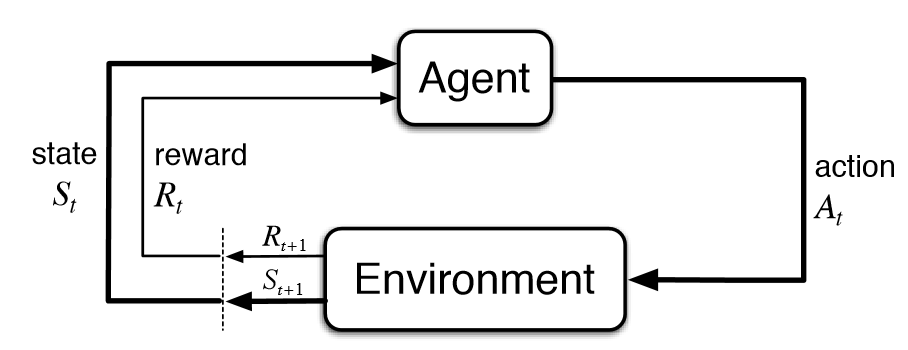
\includegraphics[max size={300}{300}]{report/assets/rl.png}
    \caption{The RL Loop}
    \label{fig:rl}
\end{figure}
\subsection{Model-Free Learning}
Model-free (or direct) RL is the traditional instantiation of RL, where the agent learns a policy directly from experience gained by interacting with the environment; it is purely trial-and-error. Model-free learning tends to be quite flexible to varying problems, since no assumptions are made about the environment's dynamics. Furthermore, since the environment's dynamics do not need to be stored, learned or considered, model-free learning is scalable and does not suffer from the \textit{curse of dimensionality} (in the non-tabular cases) and can be computationally efficient, as there is generally no lookahead deliberation process involved. However, model-free learning can be sample-inefficient; the agent may need to take many actions before discovering the optimal policy.
\subsection{Model-Based Learning}
Model-based (or indirect) RL is where an agent uses a known or learned model of the environments dynamics (in the form of an MDP) in order to learn the optimal policy \cite{MAL-086}. The agent may learn the model and policy at the same time, as in the Dyna family \cite{Sutton:1990, 10.1145/122344.122377} or learn a policy by planning over a known model, as in AlphaZero \cite{DBLP:journals/corr/abs-1712-01815} or learn a policy by planning over a learned model, as in MuZero \cite{DBLP:journals/corr/abs-1911-08265}.
Model-based learning tends to provide better sample efficiency than model-free approaches, since learning can occur from simulation rather than directly from experience \cite{RLSOTA11} and the number of exploratory actions can be reduced by using targeted exploration \cite{Thrun-1992-15850}. However, this comes at a computational cost; planning can be expensive, especially if the state and action spaces are large.
% \\Comparison
% \begin{itemize}
%     \item model-free RL is more scalable, simpler to program
%     \item model-based RL can be more efficient, can overcome delayed rewards, however comes at a cost: planning takes time and computational power.
% \end{itemize}
\subsubsection{Model Learning}
Model Learning can be a difficult problem due to uncertainty due to limited data, stochasticity and partial observability. . We omit the problem of partial observability here, since we are not considering POMDPs, however stochasticity and uncertainty are very relevant to us. Stochasticity and uncertainty can be overcome through sufficient exploration; sampling a transition multiple times can give a better estimate of the probability distribution which reduces uncertainty.
\\Model learning can be viewed as a supervised learning problem \cite{JORDAN1992307}. In discrete environments, exact models of the environment's dynamics can be learned in the form of a \textit{tabular maximum likelihood model} \cite{10.1145/122344.122377} which  maintains a table with an entry for every possible transition.
In the stochastic case, for each transition the table will store:
\begin{equation}
\label{eqn:tmlmupdate}
T(s, a, s') = \frac{n(s, a, s')}{\sum_{s'}n(s,a,s')}
\end{equation}
Where $n(s,a,s')$ represents the number of times the transition has been observed.
% The same can be used for the deterministic case, which will result in all transitions mapping to either 0 or 1. It should be noted that an environment could be discretised in order to learn an exact model, but in-fact this model will be approximate due to this discretisation.
A key drawback to this approach is the lack of scalability to large state spaces.
\\In continuous domains an exact model cannot be learned, due to the infinite number of states (and potentially actions). An approximate model can be learned by using state aggregation (which discretises the state space) and a tabular maximum likelihood model \cite{Kuvayev1996ModelBasedRL}.
However, more commonly an approximate model is learned through Function Approximation methods such as Linear Regression \cite{DBLP:journals/corr/abs-1206-3285, NIPS2007_b7bb35b9} and Gaussian Processes \cite{10.5555/3104482.3104541}.
% % However, as with all tabular methods, this doesn't scale well.
% A key drawback of this approach is the lack of scalability to large state and action spaces.
% In continuous environments, tabular approaches are not possible due to the infinite number of states and actions. However, a continuous environment's dynamics can be approximately learned using Function Approximation.


% The agent learns to act in the environment by either learning or being provided with a representation of the dynamics of the environment.
% Model-based RL is where the agent learns to act in an environment, and has some understanding of the dynamics of the environment in the form of a model. By the nature of models, the model is inaccurate, more often than not. \cite{Sutton:1990, MAL-086, 10.1145/122344.122377, Kuvayev1996ModelBasedRL, RLSOTA11}
\subsection{Temporal Difference Learning}
Temporal Difference (TD) Learning \cite{10.5555/911176, 5392560, 5391906} aims at solving the problem of temporal credit assignment by combining ideas from Monte Carlo methods, which learn directly from experience in the environment, and Dynamic Programming methods, which bootstrap estimates from other previously learned estimates. It is a form of Generalised Policy Iteration, in that it aims to produce an optimal estimate of the Value Function, $V_\pi^*$, starting from an initial estimate, $V_\pi$, for a given policy, $\pi$,\cite{Sutton1998}.
\\The core idea of TD Learning is to update the estimate of the Value Function, $V_\pi$, whenever there is a difference between temporally successive predictions \cite{Sutton:1988}. This difference is known as the TD error. The updated estimate is bootstrapped from the previous estimate, meaning that TD learning essentially learns a prediction from another prediction.
\\The simplest TD Learning algorithm is TD(0) \cite{Sutton:1988}, which updates it's estimates as such:
\begin{equation}
\label{eqn:td0update}
V(s_t) \leftarrow V(s_t) + \alpha[r_{t+1} + V(s_{t+1}) - V(s_t)]
\end{equation}
The TD target is the current prediction of the expected cumulative reward: $r_{t+1} + V(s_{t+1})$. The TD error is $r_{t+1} + V(s_{t+1}) - V(s_t)$.
$0 \le \alpha \le 1$ is the learning rate, which is used to control how much weight is given to the TD error when updating the estimate. 
\\TD Learning can also be extended to learn a Q-Function, which stores the value of state-action pairs rather than the value of states. For each state-action pair, it stores an estimate of the expected cumulative reward starting in that state and taking an action, and following a fixed policy.
% \\Starting from an initial estimate of the Value Function, $V_\pi$, for the current policy being followed, $\pi$, the goal of TD Learning is 
% \\The core idea of TD learning is to learn the optimal estimate of the Value Function of the current policy being followed. The estimate is updated whenever there is a difference between the expected reward and actual reward received at each discrete time step; learning occurs whenever there is a difference between temporally successive predictions.
% The core idea of TD learning is to maintain an estimate of the Value Function of the current policy being followed, this estimate is updated whenever there is a difference between temporally successive predictions; this difference is known as the TD error.
% TD Learning algorithms can be on-policy, such as SARSA \cite{rummery:cuedtr94}, where the value of the policy being currently carried out by the agent is learnt, or off-policy, such as Q-Learning \cite{Watkins:1989, journals/ml/WatkinsD92}, where the value of the optimal policy is learnt independently of the agent's actions following the current policy.
% \cite{PooleMackworth17}.


% Within Temporal Difference (TD) \cite{10.5555/911176, 5392560, 5391906}, learning is driven by the error/difference between temporally successive predictions, so learning occurs whenever there is a change in prediction over time. It's a method for learning to predict; learning a prediction from another later learned prediction.
% The problem of temporal credit assignment gives rise to Temporal Difference (TD) Learning \cite{10.5555/911176, 5392560, 5391906}. TD Learning maintains an estimate of the Value Function, which is updated whenever there is a change in prediction over time.
\subsubsection{Q-Learning}
Q-Learning \cite{Watkins:1989, journals/ml/WatkinsD92} is an off-policy TD Learning method that learns a Quality function. It is off-policy, as the update rule assumes a greedy policy - this means that the value of the optimal policy is learned independently of the agent's actions following the current policy. Q-values are iteratively updated using the Bellman equation, the update rule is as follows:
\begin{equation}
\label{eqn:qlearningupdate}
Q(s_t,a_t) \leftarrow Q(s_t,a_t) + \alpha[r_{t+1} + \max_aQ(s_{t+1}, a) -Q(s_t,a_t)]
\end{equation}
Where $0 \le \alpha \le 1$ is the learning rate, which indicates how quickly learning occurs.
% \\Clearly Q-Learning comes from Dynamic Programming, and in that sense it is a tabular method; a Q-table is maintained which stores the Q-values for each state-action pair. For this reason, it doesn't scale too well to large state/action spaces - however it is suitable for the domains that we consider within this work.
% \\The result of Q-Learning is that a deterministic, greedy policy is learned.
\subsubsection{SARSA}
SARSA (State Action Reward State Action) \cite{rummery:cuedtr94} is an on-policy TD Learning method that learns a Quality function. It is on-policy, as the update rule assumes that the current policy continues being followed - this means that the value of the current policy being followed is learned. Q-values are iteratively updated using the Bellman equation, the update rule is as follows:
\begin{equation}
\label{eqn:sarsaupdate}
Q(s_t, a_t) \leftarrow Q(s_t, a_t) + \alpha[r_{t+1} + Q(s_{t+1}, a_{t+1})-Q(s_t, a_t)]
\end{equation}
Where $0 \le \alpha \le 1$ is the learning rate, which indicates how quickly learning occurs.
\subsection{Exploration in Reinforcement Learning}
Thrun \cite{Thrun-1992-15850} distinguished exploration methods in to two main categories: directed and undirected. Directed exploration refers to exploration that is informed by memory about the state space, whereas undirected exploration is uninformed, random. More recently, Amin, et al. \cite{DBLP:journals/corr/abs-2109-00157} presented a comprehensive survey on exploration in RL, which distinguished between reward-free and reward-based exploration; each of these categories is then broken down into memory-free (undirected) and memory-based (directed) exploration. However, we prefer to distinguish between model-free and model-based exploration. Model-free methods tend to be classical methods, and more often than not employ randomness whereas model-based methods are mostly more advanced, and may use planning, intrinsic motivation and curiosity to explore.
\subsubsection{Model-Free Exploration}
% Model-free approaches to exploration are often chosen, due to their simplicity of implementation, scalability and robustness to diverse domains. Generally, no modifications need to be made to a model-free exploration approach when deploying it in different domains.
Purely random exploration comes in the form of a Random Walk, or unguided random search \cite{anderson86}, which arises from randomly sampling actions with uniform probability, as seen in Equation \ref{eqn:rw}. 
\begin{equation}
\label{eqn:rw}
    a_t \sim P(A)
\end{equation}
Where $P(A)$ is the uniform distribution over the action space, $A$. Exploration occurs naturally when the agent moves away from the goal, rather than closer to it, due to the uniform selection of actions. This is perhaps the most naive method of exploration, since it is entirely random and is therefore very inefficient.
\\$\epsilon$-greedy \cite{Watkins:1989, conf/nips/Sutton95} uses a hyperparameter, $\epsilon$ to balance between exploration and exploitation. With probability $\epsilon$ the agent explores by taking a random action, which is sampled with uniform probability, with probability $1-\epsilon$ the agent exploits by taking the best action, which is selected greedily with respect to the current policy; this is summarised in Equation \ref{eqn:egreedy}.
\begin{equation}
\label{eqn:egreedy}
a_t = 
\begin{cases}
\pi(s_t) \qquad \qquad \qquad \text{with probability} \quad 1-\epsilon\\
\text{random action} \qquad  \text{with probability} \quad $\epsilon$
\end{cases}
\end{equation}
Where $0 \le \epsilon \le 1$, and $\pi$ is the current greedy policy.
Whilst this provides a clear method for balancing exploration and exploitation, it lacks temporal persistence. Furthermore, by the nature of the name, it is a greedy method which could lead to a local optima. $\epsilon$ may be decayed temporally, to ensure that lots of exploration happens early on, and then exploitation occurs more when learning has occurred. Whilst $\epsilon$-greedy is very easy to implement, it is very inefficient and only converges to optimality in the limit, under certain conditions.
\\$\epsilon z$-greedy \cite{dabney2021temporallyextended} is an extension to $\epsilon$-greedy that uses temporal persistence. The agent follows a temporally-extended sequence of actions with probability $\epsilon$ and with probability $1-\epsilon$ exploits by taking the best action, which is selected greedily with respect to the current policy. The temporally-extended sequences of actions are called options \cite{SUTTON1999181}). The options consist of actions repeated $n$ times, where $n$ is chosen from a distribution. Whilst this overcomes some of the issues with $\epsilon$-greedy, it can suffer in complex MDPs, where long exploratory trajectories which result in nothing informative being learned can be a very big waste of time and resources.
\\ Boltzmann exploration samples an action according to the Boltzmann distribution:
\begin{equation}
\label{eqn:boltzmann}
\pi(a|s) = \frac{e^{Q(s,a)/\tau}}{\sum_{a' \in A}e^{Q(s,a')/\tau}}
\end{equation}
Where $\tau$ is the temperature, and determines how frequently random actions are chosen. As $\tau$ decreases, the policy approaches greediness \cite{DBLP:journals/corr/cs-AI-9605103, DBLP:journals/corr/abs-2109-00157}. $\tau$ may be decayed temporally, in the same fashion as $\epsilon$ can be decayed temporally in $\epsilon$-greedy. Here we gave the definition in the context of a $Q$-function, however this can be replaced with any value that estimates the reward received from taking action $a$. The main drawback of this approach is that the initial value for $\tau$ needs to be carefully selected, and may need to be tuned for each environment. This is because as $\tau$ approaches 0 the agent acts greedily, whereas at large values of $\tau$, all actions have an approximately uniform probability of being selected leading to exploration akin to a Random Walk \cite{DBLP:journals/corr/abs-2109-00157}.
\\ Whilst these model-free approaches are useful, in that they are generally easy to implement and are robust to varying domains, they tend to share two common drawbacks: practical inefficiency and introducing additional hyperparameters that have to be tuned. Furthermore, their lack of reasoning implies a lack of intelligence.
% \\Optimistic Initial Values
\subsubsection{Model-Based Exploration}
Explicit Explore or Exploit ($E^3$) \cite{Kearns+Singh:2002} maintains a partial model of the environment through collecting statistics, akin to the \textit{tabular maximum likelihood} approach. A distinguishement is made between \textit{known} and \textit{unknown} states; a state is \textit{known} after it has been visited an arbitrary number of times, thus its learned dynamics must be close to the true dynamics. If the current state is \textit{unknown}, then \textit{balanced wandering} takes place, and the agent explores by selecting the action that has been taken the least number of times from that state. If the current state is \textit{known} then the action is chosen greedily with respect to the current model.
\\ R-MAX \cite{10.1162/153244303765208377} is an extension and generalisation of $E^3$. It begins with an optimistic initial model such that every transition leads to some imaginary state that returns the maximal reward, denoted $R_{max}$. R-MAX uses the same concept of \textit{known} and \textit{unknown} states as in $E^3$; after a state becomes known, then the model is updated with the collected statistics regarding that state. The agent always follows the optimal policy according to the model. R-MAX removes the need for explicit contemplation between exploring and exploiting as in $E^3$; exploration and exploitation occur naturally.
\\ Optimistic Initial Model (OIM) \cite{10.1145/1390156.1390288} begins with an optimistic model, the same as R-MAX. The model is updated through observations similarly to $E^3$. The agent maintains two Q-functions, $Q^r$ and $Q^e$, which are initialised and updated according to observations through dynamic programming. $Q^r$ corresponds to the "real", extrinsic rewards, whereas $Q^e$ corresponds to the intrinsic exploration rewards. Whilst exploring, the agent acts optimally with respect to the combination of the two Q-functions; thus $Q^e$ can be seen as an exploration bonus. During this, the agent will either act near-optimally, or will gain new information it can utilise. After exploration is terminated, $Q^e$ is dropped and the agent acts optimally with respect to $Q^r$.
\\ $E^3$, R-MAX and OIM are provably able to achieve near-optimal performance in polynomial time, however they are limited to full-observability and discrete environments. Furthermore, although the optimistic stance taken in R-MAX and OIM leads to good exploration, it is misplaced in a sense, since it is very likely and maybe impossible that any of the optimism comes to fruition.
\\ Model-Based Active Exploration (MAX) \cite{DBLP:journals/corr/abs-1810-12162} is purely an exploration framework, which pure exploitation could follow from. An ensemble of dynamics models is maintained and trained, and within each episode a model is sampled from the ensemble, and a policy is derived from the model such that it maximises the intrinsic reward function which is based on the Jensen-Shannon Divergence. The agent then explores by following this policy. Exploration is task-agnostic, which means it generalisation to downstream tasks is a possibility. However, due to the ensemble-based approach, is is quite computationally inefficient.
\\ Plan2Explore \cite{plan2explore} is a task-agnostic framework that separates learning in to two separate phases. During the first phase, the agent explores via planning and intrinsic motivation in order to learn an accurate model of the environment, in the form of a latent dynamics model. In the second phase, the agent uses extrinsic reward to adapt to a specific task. A notable achievement of Plan2Explore is its ability to easily adapt to downstream tasks in high-dimensional environments. However, the exploration and model-training loop is very complex, and could potentially be quite slow computationally.
\\Planning Exploration Goals (PEG) \cite{hu2023planning} performs exploration by sampling states by intrinsic motivation, and then exploring by planning to those states. Exploration is task-agnostic.
\\ GoExplore \cite{goexplore}
\\While MAX, Plan2Explore, PEG and GoExplore achieve task-agnostic exploration that allows fast, and in some cases zero-shot, adaptation to downstream tasks in high-dimensional and continuous domains, they do this at a very large computational cost due to their nature.
\\Domain Approximation for Reinforcement Learning (DARLING) \cite{AIJ16-leonetti} computes a \textit{partial policy} from the model, using the planner. A \textit{partial policy} is a function that maps states to possible actions, and is constructed from a subset of possible plans according to some metric and threshold (for instance all plans that are shorter than 1.5 times the length of the shortest plan). RL is then done inside the partial policy through $\epsilon$-greedy. This leads to constraining exploration to a set of seemingly reasonable states, enabling the agent to overcome inaccuracies in the model, although the model is not explicitly learned. The main problem in this approach, is that it is only suitable for where the inaccuracies are not too significant, so there is a reliance on the embedded model being somewhat correct; as if the optimal policy does not exist in the partial policy, it will never be discovered. A key benefit of this approach is the ability to constrain exploration through reasoning, whilst also being able to scale to stochastic, continuous domains, such as a real world robotics navigation task. However, the use of $\epsilon$-greedy introduces randomness into the framework. DARLING is perhaps the work closest related to ours, because it leverages human knowledge in the model, whereas the other approaches tend to learn the model entirely from scratch.
\\A common assumption among the aforementioned methods is that the model will eventually become correct, which is often not the case especially in complex tasks. Furthermore, human knowledge is often not leveraged in the form of a model, which means learning takes place from scratch. Whilst this done mean that the agents do not have to worry about model inaccuracies, it means they do not leverage useful information that can be present in models created by humans. The outlier to these drawbacks is DARLING, which makes it perhaps the most related work to ours. DARLING puts some trust in the model to guide exploration, but acknowledges that it is likely inaccurate and therefore only uses it for that - the optimal policy is discovered through learning. The approach we take is similar; we put some trust in the model, that there is some useful information embedded in there, but ultimately acknowledge that it is probably not entirely correct and thus only use it to guide exploration.


% All models are useful, but none are correct.


% Whilst learning from scratch means that the agents do not have to worry about model inaccuracies, it means that the agents are missing useful
% \section{Exploration in Reinforcement Learning}

% \subsection{Random Exploration}
% % Due to simplicity of implementation and ease of generalisation, random exploration is the most popular form of exploration, and is widely seen in the literature; even where some other exploration method is used, there is often some underlying randomness.

% % The agent only explores and doesn't exploit; unless it learns a value function whilst exploring which it switches to exploit after some number of discrete time steps.

% % $\epsilon$-greedy that uses temporal persistence; the agent follows a temporally-extended sequence of actions (an option \cite{SUTTON1999181}) until termination with probability $\epsilon$ and with probability $1-\epsilon$ the agent exploits by taking the current best action.
% % \begin{itemize}
% %     \item Pure random exploration: Random Walk
% %     \item $\epsilon$-greedy \cite{Watkins:1989, conf/nips/Sutton95}
% %     \item $\epsilon z$-geedy \cite{dabney2021temporallyextended, SUTTON1999181}
% %     \item Softmax
% %     \item Boltzmann \cite{Watkins:1989, 10.1007/BF00992699, SCC.Barto.Bradtke.ea1991}
% % \end{itemize}
% % \subsection{Intrinsically Motivated Exploration}
% % \cite{scott1996, pmlr-v97-jinnai19b, Jinnai2020Exploration}
% % \subsection{Optimistic}
% % \cite{10.1145/1390156.1390288, NIPS2006_c1b70d96, 10.1162/153244303765208377, NIPS2008_d5cfead9}
% \subsection{Model-based}
% Not all model-based RL methods use models as part of their exploration, therefore model-based exploration methods are a subset of model-based RL.
% % Planning-based approaches are by definition model-based. We consider any model-based approach to utilise planning-based exploration if the 
% % We refer to Model-Based exploration as any method of exploration that uses a model to influence exploration.

% % \cite{SARA07-jong}

% % For instance, a simple form of model-based RL where an agent plans on an initial model, and performs model-learning concurrently is an exploration method; although a naive one, that doesn't work in practice.\\
% % \cite{SARA07-jong, Littman2011EfficientME, Epshteyn2008ActiveRL}
% % \subsubsection{DARLING}
% \\ Plan2Explore \cite{plan2explore} explores using planning and intrinsic motivation to learn a model of the world. Exploration is task-agnostic, this leads to the agent learning the dynamics of the world, and being able to transfer to downstream tasks easily.
% \\ MAX \cite{DBLP:journals/corr/abs-1810-12162} explores using planning and intrinsic motivation. It aims to seek out novel states by Jensen-Renyi Divergence \cite{renyi}.
% \\DARLING \cite{AIJ16-leonetti} approximates a deterministic model, which it then produces a partial policy from which $\epsilon$-greedy is performed within. A partial policy is essentially a combination of a selection of plans.  This leads to constraining exploration to a set of seemingly reasonable states, enabling the agent to overcome inaccuracies in the model, although the model is not explicitly learned. The main problem in this approach, is that it is only suitable for where the inaccuracies are not too significant, so there is a reliance on the embedded model being somewhat correct. Also, DARLING is only suitable for domains where discretisation is possible; it does not scale to continuous state or action spaces. Furthermore, $\epsilon$-greedy introduces randomness into the framework.
% \\ LEO \cite{10.5555/2484920.2485088} learns the best exploration strategies on-line, given a set of exploration strategies. It chooses those which discover rewards and goal quickest; thus lead to the most efficient exploration.
% \\ OIM \cite{10.1145/1390156.1390288} uses an overly optimistic model, which is updated and learned approximately through experience, to guide exploration by greedily acting with respect to a value function computed through dynamic programming.

% \\ R-MAX \cite{10.1162/153244303765208377} begins with a model of the environment which assumes that all transitions lead to a hypothetical maximum-reward terminal state. The model is updated through experience. The optimal policy with respect to the model is either near optimal in the real environment, or useful because it leads to learning.

% \\Fitted R-MAX \cite{SARA07-jong} is an extension of R-Max to continuous domains.
% \\ \cite{NIPS2008_d5cfead9}
% \\ DOVE \cite{pmlr-v120-seyde20a}
% \\ $E^3$ \cite{Kearns+Singh:2002}
% \\ \cite{10.1016/S0004-3702(98)00002-2}
% \\ \cite{10.5555/2886521.2886686}
% \\ \cite{ISHII2002665}
% \\ \cite{NIPS2012_a0a080f4}
% \\ \cite{10.1145/1553374.1553441}
% \\ \cite{10.1145/1143844.1143932}
% \\ \cite{10.1145/1143844.1143845}

% \subsubsection{PEORL}
% PEORL \cite{DBLP:journals/corr/abs-1804-07779}
% \subsubsection{Plan-Q Learning}
% \cite{10.1007/978-3-540-77949-0_6}
% \subsubsection{FRAP}
% \cite{DBLP:journals/corr/abs-2006-15009}
% \subsubsection{Guided Dyna-Q}
% \cite{Hayamizu2021GuidingRE}
% \subsubsection{TMP}
% \cite{Jiang2019TaskMotionPW}
% \subsubsection{Simple Model-Based Exploration}
% For benchmarking and comparison purposes, we present a simple model-based exploration method.
% \begin{figure}[h!]
%     \centering
%     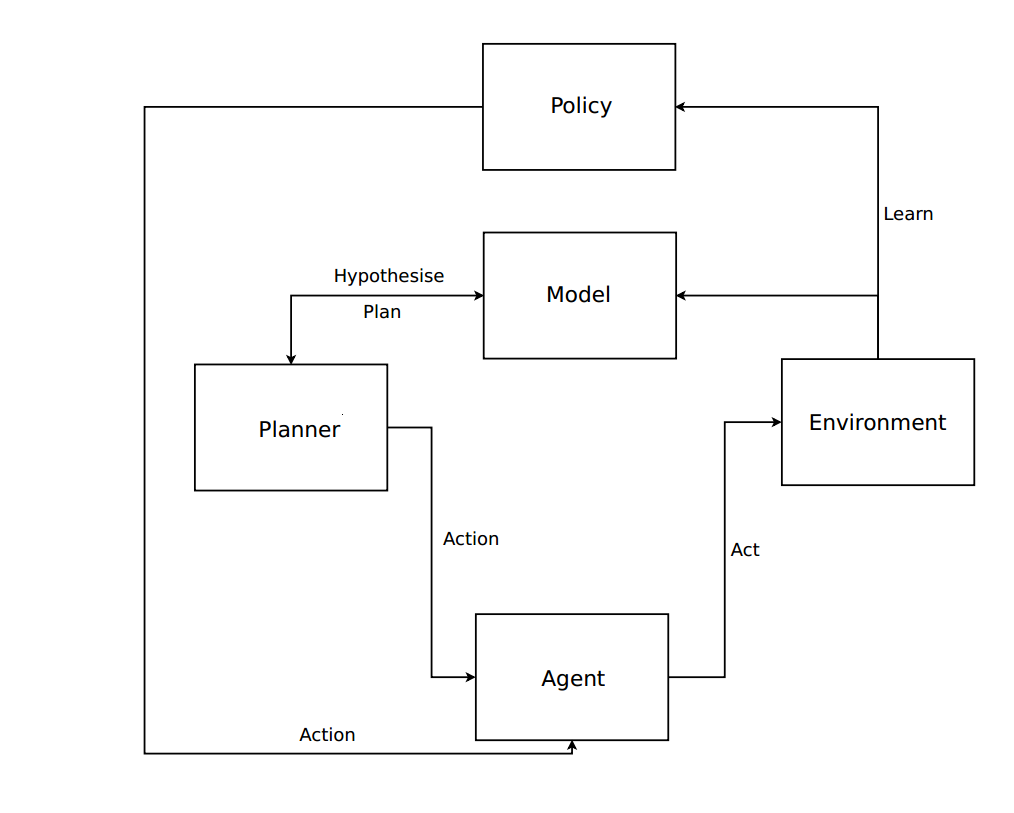
\includegraphics[max size={\textwidth}{\textheight}]{report/assets/diagram.png}
%     \caption{Framework}
%     \label{fig:framework}
% \end{figure}
% Randomnes underlies most exploration strategies in RL, from using pure-randomness, to randomly samplin
% \subsection{Random}
% \subsubsection{$\epsilon$-greedy}
% $\epsilon$-greedy \cite{Watkins:1989, conf/nips/Sutton95} aims to balance exploration and exploitation through an $\epsilon$ factor, such that the agent exploits its learned knowledge, taking the current best action, with probability $1-\epsilon$ and explores randomly with probability $\epsilon$. It's common to decay $\epsilon$ temporally, so that the agent explores a lot early on and then exploits more after it has learnt for a while. Whilst this method offers a nice balance between the two extremes of pure exploration and pure exploitation, it only provably converges to an optimal policy with an infinite number of observations, so in-fact it is quite inefficient. Furthermore, due to the random nature, it results in continually evaluating sub-optimal actions. A key drawback to $\epsilon$-greedy is that without infinite observations, it can easily get stuck in a local optima.
% \subsubsection{$\epsilon z$-greedy}
% Dabney, et al., \cite{dabney2021temporallyextended} stated that another key problem with $\epsilon$-greedy is its lack of temporal persistence; actions are only performed for one time-step. They proposed $\epsilon z$-greedy, or temporally extended $\epsilon$-greedy, where the agent takes the current best action with probability $1-\epsilon$ and follows an "option" until termination with probability $\epsilon$. An "option" is a sequence of actions, akin to a "plan" in the planning literature.
% \subsubsection{Boltzmann}
% \subsubsection{Thompson Sampling}
% \subsubsection{UCB}
% \subsubsection{Conclusion}
% \subsection{Intrinsically Motivated}
% \subsubsection{Count-based}
% \subsubsection{Information Theoretic}
% \subsubsection{Curiosity Driven}
% \subsection{Model-Based Exploration}
% \subsubsection{DARLING}
% Leonetti et al \cite{AIJ16-leonetti}, developed DARLING (Domain Approximation for Reinforcement Learning), where given a model, a planner is used to produce a "partial policy", which is a set of reasonable choices the agent can make in each state. Exploration is then constrained to this partial policy, and performed using $\epsilon$-greedy. This work showed that whilst planning and RL take two different approches to decision making, on on their own each struggle in stochastic, high-dimensional domains, integrating them can overcome each of their weaknesses. This work was successful in carrying out complex robotics tasks, even with an inaccurate model, and moreover, it showed that the region of the environment that is explored by the agent is more reasonable and is goal-directed.
% \subsection{Evaluating RL}
% When studying and developing algorithms, its important that firstly they work but secondly that they work efficiently. Generally, the efficiency of algorithms is measured by their time and space complexity; which indicates how the time and space requirements of the algorithm increase as the size of the input increases. In RL, we are mostly interested in sample complexity, which refers to how many interactions are required with the environment in order to effectively learn \cite{Kakade2003OnTS}. The sample complexity of exploration refers to how many sub-optimal actions are followed during learning.


% \\In the context of RL, sample complexity refers to how much data (how many interactions with the environment) we need to collect in order to learn, and the computational complexity refers to how much computation needs to be performed using this data to learn .




% \subsection{Learning Curves}
% \subsection{Varying Domains}
\\
\\
% \\PAC, Regret \cite{lattimore}, Learning curve
% \subsubsection{What is "Efficient Exploration"?}

% \cite{10.5555/1867270.1867286, 10.5555/1577069.1755867, Kakade2003OnTS}